
%%Textinhalt
\chapter{Ausgeben von Signalen}

\section{Durchf\"uhrung}
In dieser Aufgabe sollte der DSP ein Sinussignal generieren. Die Frequenz sollte 
dabei per Taster in 200Hz Schritten einstellbar sein. 
Die drei auf dem DSP angebrachten LEDs sollten die Frequenzen 200Hz, 400Hz und 4kHz darstellen.

Zur Realisierung dieser Aufgabe wurde in der Vorbereitung eine Funktion genSinus erstellt, 
die bei jedem Aufruf den nächsten Wert des Sinussignals ausgibt.

\begin{adjustbox}{width=\textwidth,keepaspectratio}
\lstinputlisting[title=gensinus.c]{gensinus.c}
\end{adjustbox}\pagebreak

Die Funktion ist so Implementiert, dass sie den jeweiligen Zeitpunkten einen entsprechenden Sinuswert zuweist und diesen zurückweißt. 
Als \"Ubergabeparameter sind zum einen die Amplitude und zum anderen die Frequenz vorgesehen, wobei die Frequenz in 200Hz Schritten \"ubergeben wird. 

Das neue \begin{math}\omega_{Norm}\end{math}, also wird entsprechend mit 
\begin{equation}\label{normierteKreisfrequenz}
 \omega_{Norm}=2\pi*f 
\end{equation}  
ermittelt und normiert.\\\par
Der Aufruf durch den Timer-Interrupt stellt dabei die Periodizität sicher. 
Das alte \begin{math}\omega_{Norm}\end{math} wird dann mit dem neuen \begin{math}\omega_{Norm}\end{math} addiert und mit der Funktion sin aus math.h 
wird der entsprechende Sinuswert ermittelt. Die Skalierung erfolgt durch Multiplikation mit A, da sin() einen Normierten Wert zwischen 0 und 1 zurückgibt.

Um die LEDs und Taster entsprechend nutzen zu können wurde die main.c angepasst.
\begin{adjustbox}{width=\textwidth,keepaspectratio}
\lstinputlisting[title=main.c]{main2.c}
\end{adjustbox}\pagebreak

Da auf die Eingabe der Taster reagiert werden soll, musste die \gls{isr} angepasst werden.
Dazu wird in einer Switch-Case-Anweisung überprüft welche Frequenz eingestellt 
wurde.\par
\begin{adjustbox}{width=\textwidth,height=\textheight,keepaspectratio}
 \begin{lstlisting}[title=isr.c]{isr.c}
    if (Freq200 == 1)
        *pFIO2_FLAG_S = 0x0100;
    // !! set control register so that LED 5 is on
    else if (Freq200 == 2)
        *pFIO2_FLAG_S = 0x0200;
    // !! set control register so that LED 6 is on
    else if (Freq200 == 20)
        *pFIO2_FLAG_S = 0x0400;
    // !! set control register so that LED 7 is on
    else
        *pFIO2_FLAG_C = 0x0700;
    // !! set control register so that no LED is on
    
     ssync();

    // copy sine value to dma output buffer
    iDMATxBuffer[4] = genSinus(AMPLITUDE, Freq200) * LONG_MAX;   
\end{lstlisting}
\end{adjustbox}

Entsprechend der Aufgabe wurden die LEDs gesetzt sobald die entsprechende Frequenz 
ausgewählt ist. Dies wird mit der \gls{pf}\textunderscore S realisiert. \textunderscore S steht in diesem Fall für set.
Ist keine der im Switch-Case angegebenen Frequenzen ausgewählt, so wird die \gls{pf} mit dem Prefix \textunderscore C zurückgesetzt, \textunderscore C steht für clear.

Im Array iDMATxBuffer steht am Index 4 der 32bit Ausgabewert des DAC, 
da die Funktion genSin() nur Werte zwischen -1 und 1 zurück gibt wird mit dem 
maximalen Wert des 32-bit Formats multipliziert(definiert als LONG\textunderscore MAX). 
Dies ermöglicht die Ausnutzung des gesamten Spannungsbereiches des DAC.


Das Board wurde in Betrieb genommen und für die Frequenzen 200Hz, 
400Hz und 4kHz wurden sowohl Spannungs-Zeit Verläufe als auch Spektren mit Hilfe des \gls{vi} aufgenommen. 
Auf Grund von Unachtsamkeit ist das Bild des Spektrums des 200Hz Signals verloren gegangen und kann hier daher nicht gezeigt werden.

Wir rekonstruieren aus unseren Unterlagen, dass es wie erwartet aussah und auf kein besonderes Verhalten hinwies.

\pagebreak
\section{Auswertung}



Für eine Vergleichbarkeit der Signale haben wir alle Bilder der Signale (Abbildung \ref{fig:Scope200Hz} bis \ref{fig:Scope4kHz}) 
der gleichen Auflösung für Amplitude und demselben Level für den Trigger erzeugt. 
Die Zeitbasis wurde entsprechend angepasst, sodass vier Perioden zu sehen 
sind.\\\par
Die Resultate entsprechen den Erwartungen, wobei die Amplitude von 0,7V anfangs überraschte. 
Die Amplitude ergibt sich aus dem Hardwareaufbau des \gls{evb}, so liegt die maximale Aussteuerung bei 6,17V Spitze-Spitze des Codec, was zu einer maximalen Amplitude von 3,08V 
führt.
Softwareseitig haben wir die Amplitude so eingestellt, dass sie das Signal genau auf die Hälfte skaliert, dies erzeugt eine Amplitude von ca. 1,5V.
Allerdings lassen sich nur 0,7V messen, da die Ausgangsstufe des \gls{evb} einen Spannungsabfall hat.
\begin{figure}[h!]
  \centering
    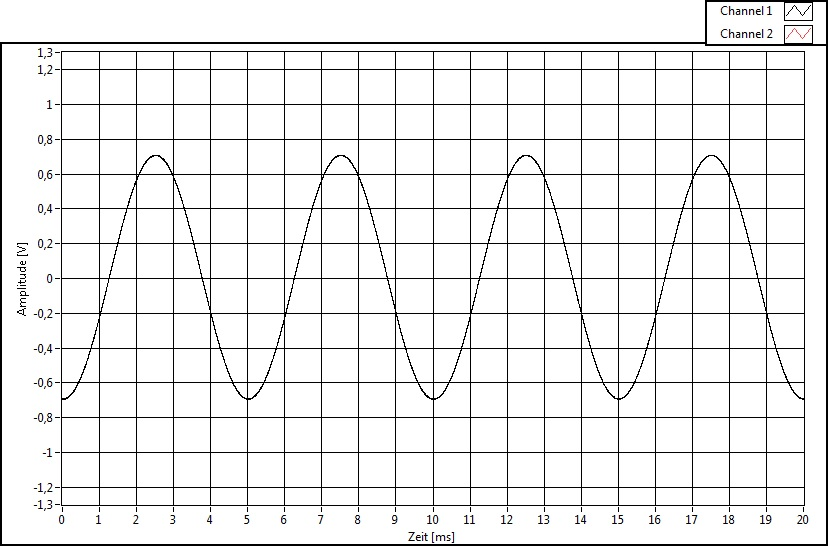
\includegraphics[width=\textwidth]{200Hz.jpg}
  \caption{Spannungs-Zeit Verlauf 200Hz}
  \label{fig:Scope200Hz}
\end{figure}
\begin{figure}[t!]
  \centering
    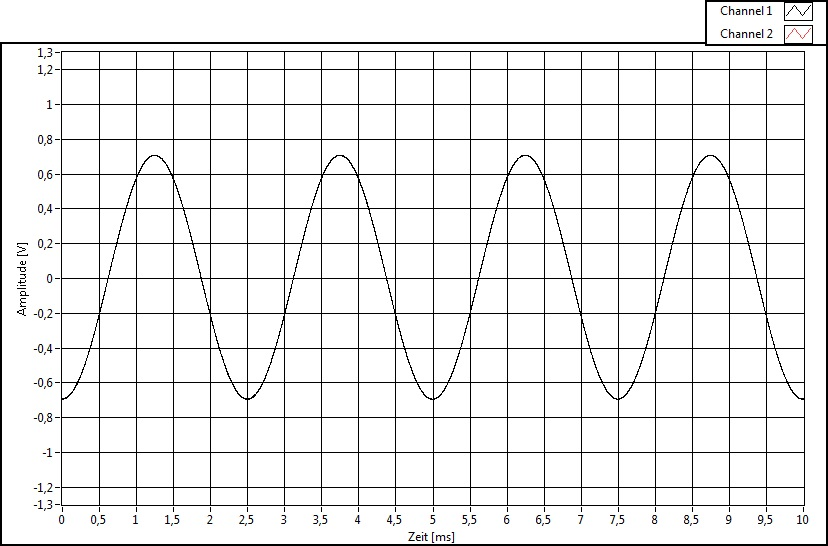
\includegraphics[width=\textwidth]{400Hz.jpg}
  \caption{Spannungs-Zeit Verlauf 400Hz}
  \label{fig:Scope400Hz}
\end{figure}
\begin{figure}[b!]
  \centering
    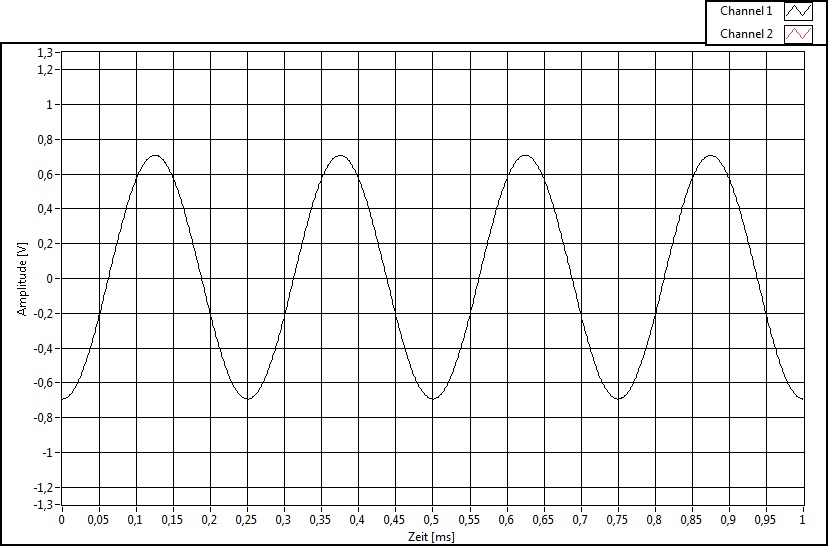
\includegraphics[width=\textwidth]{4kHz.jpg}
  \caption{Spannungs-Zeit Verlauf 4kHz}
  \label{fig:Scope4kHz}
\end{figure}\\\par
Die Spektren sehen genau wie erwartet aus und zeigen bei der entsprechend eingestellten Frequenz einen entsprechenden Peak. 
Einige kleine Peaks sind bei anderen Frequenzen zu ermitteln, ihre Höhe ist aber im Verhältnis so gering, dass sie vernachlässigt werden können.
\begin{figure}[bp!]
    \centerline{
    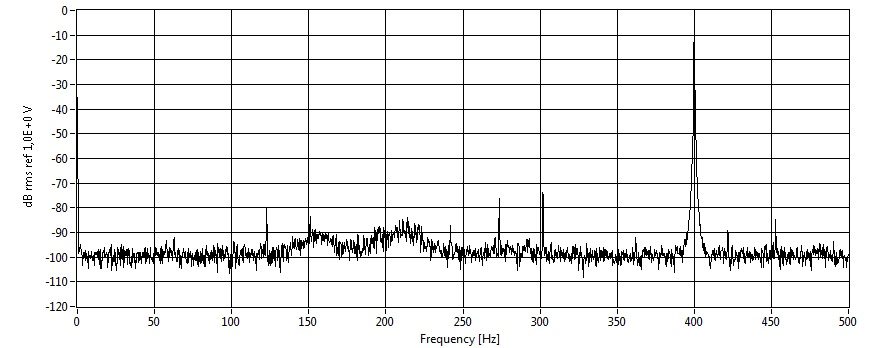
\includegraphics[width=\textwidth]{FFT400Hz.jpg}}
  \caption{Amplitude(dB)-Frequenz Verlauf 400Hz}
  \label{fig:FFT400Hz}
\end{figure}
\begin{figure}[bp!]
  \centering
    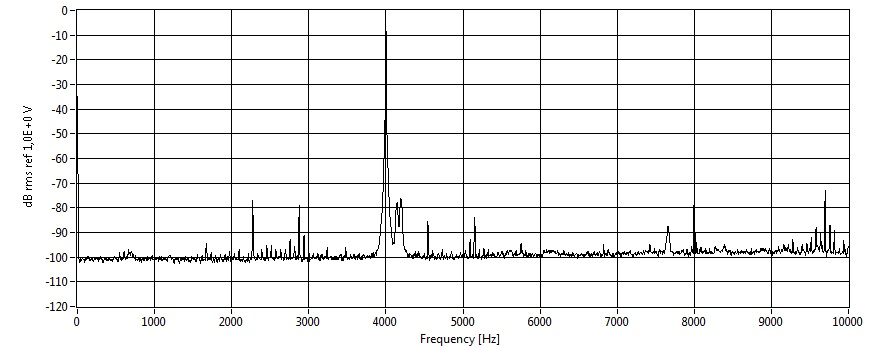
\includegraphics[width=\textwidth]{FFT4kHz.jpg}
  \caption{Amplitude(dB)-Frequenz Verlauf 4kHz}
  \label{fig:FFT4kHz}
\end{figure}


